\documentclass[border=6pt]{standalone}
\usepackage{tikz}
\usepackage[edges]{forest}
\usetikzlibrary{arrows.meta,positioning,calc,decorations.pathreplacing,shapes.geometric}
\begin{document}
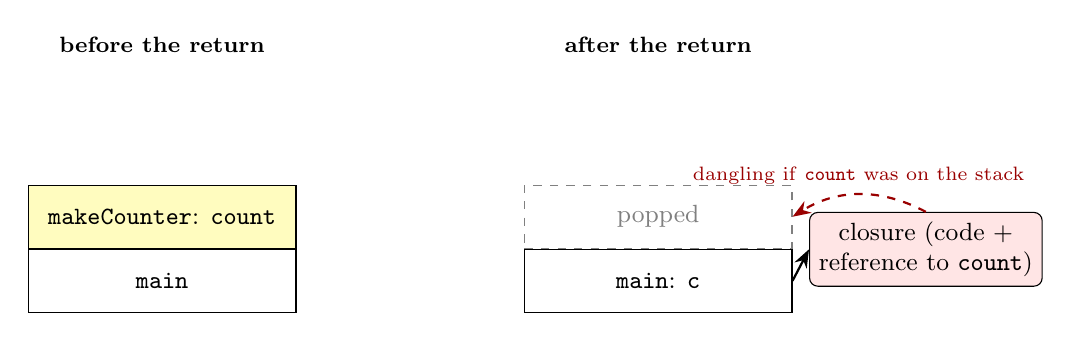
\begin{tikzpicture}[>=Stealth,font=\small,
 rec/.style={draw,minimum width=3.4cm,minimum height=0.8cm,align=center}]
\node[font=\footnotesize\bfseries] at (1.7,3.0) {before the return};
\node[rec] (m1) at (1.7,0) {\texttt{main}};
\node[rec,above=0cm of m1,fill=yellow!25] (mc) {\texttt{makeCounter}: \texttt{count}};
\node[font=\footnotesize\bfseries] at (8.0,3.0) {after the return};
\node[rec] (m2) at (8.0,0) {\texttt{main}: \texttt{c}};
\node[rec,above=0cm of m2,dashed,gray] (mc2) {popped};
\node[draw,rounded corners=3pt,fill=red!10,minimum width=2.6cm,align=center] (cl) at (11.4,0.4) {closure (code +\\reference to \texttt{count})};
\draw[->,thick] (m2.east) -- (cl.west);
\draw[->,thick,red!60!black,dashed] (cl.north) to[bend right=30] node[above,font=\scriptsize]{dangling if \texttt{count} was on the stack} (mc2.east);
\end{tikzpicture}
\end{document}
